% Postmortem of the NL = UL formalization (issue #6747).
% Build: tectonic postmortem.tex   (or: xelatex postmortem.tex, run twice)
% Data: cum.dat and hourly.dat are produced by collect.py from the public GitHub record.
\documentclass[11pt]{article}
\usepackage[a4paper,margin=2.3cm]{geometry}
\usepackage{fontspec}
\usepackage{microtype}
\usepackage{amsmath,amssymb}
\usepackage{booktabs,tabularx,array}
\usepackage{xcolor}
\usepackage{tikz}
\usetikzlibrary{arrows.meta,positioning,fit,calc}
\usepackage{pgfplots}
\pgfplotsset{compat=1.18}
\usepackage{enumitem}
\setlist{itemsep=1pt,topsep=3pt}
\usepackage[section]{placeins}
\usepackage[hidelinks]{hyperref}
\usepackage{caption}
\captionsetup{font=small,labelfont=bf}
\usepackage[skins,breakable]{tcolorbox}

\definecolor{c1}{HTML}{2C6FAC}
\definecolor{c2}{HTML}{D9822B}
\definecolor{c3}{HTML}{3F9E5A}
\definecolor{c4}{HTML}{B5443B}
\definecolor{grayf}{HTML}{EEEEEE}

\newcommand{\pr}[1]{\href{https://github.com/cslib-community/cslib-frontier/pull/#1}{\##1}}
\newcommand{\iss}[1]{\href{https://github.com/cslib-community/cslib-frontier/issues/#1}{\##1}}
\newcommand{\code}[1]{\texttt{\small #1}}
\newcolumntype{L}{>{\raggedright\arraybackslash}X}

\title{Formalizing a five-page paper in two days:\\
a postmortem of NL\,=\,UL in cslib-frontier}
\author{cslib-frontier contributors\thanks{Prepared by an agent from the public GitHub record of
issue \iss{6747} and its 209 linked pull requests, plus aggregate local operating logs where
stated. Reviewed in five rounds by an independent agent reader. Measurements are dated
22 November 2026.}}
\date{22 November 2026}

\begin{document}
\maketitle

\begin{abstract}
\noindent cslib-frontier contributors formalized Hoza's NL\,=\,UL paper (ECCC TR26-323; five pages,
seven with references) in 47.7 hours, through 209 pull requests and about 40\,000 lines of Lean. About a
tenth of the code is the paper's own argument. The rest proves what the paper cites or treats as
routine, chiefly the Reinhardt--Allender algorithms and space-bounded machine implementations of
every step. Independent components parallelized well. The time went to integrating dependent layers
one at a time, and to a 12-hour final tail caused by a misdiagnosed source check and an agent
outage. With batched integration and earlier source checks, about 35 hours looks achievable.
\end{abstract}

\section*{Summary}

\paragraph{What was done.} The paper proves two theorems.
\begin{itemize}
\item \textbf{Theorem~1.3} (about two pages) gives a generator. A seed of logarithmic length
determines vertex weights, and for some seed every connected pair of vertices in a layered graph
has a unique minimum-weight path.
\item \textbf{Theorem~1.1}, NL\,=\,UL, then follows in three bullets that cite Reinhardt and
Allender~[RA00]. NL is the class of problems decided by nondeterministic machines with
logarithmic work space. UL is the subclass where, in addition, every input has at most one
accepting run.
\end{itemize}
The formalization proves both theorems for concrete Turing machines. Space is bounded on every
partial run, including rejecting ones, and unambiguity is an exact count of accepting runs. Both
landed on \code{main}: Theorem~1.1 via \pr{7163} at hour~47.0, and Theorem~1.3 via \pr{7476} at
hour~47.7. Hour~0 is the opening of issue \iss{6747}, 20 November 14:57 UTC. Terms in
italics are explained in the Glossary below.

\paragraph{What worked.}
\begin{itemize}
\item The proof route never changed.
\item Machine-model interfaces were fixed in the first hours; dozens of components then
proceeded in parallel: 62 PRs merged by hour~14, with a median of 1.3~hours from opening to merge.
\item A claim protocol kept almost all work unduplicated.
\item Review caught a real compiler defect and a citation error.
\item Mechanically verified \emph{rollups}, single PRs that bundle several approved PRs, cleared a
large backlog in ten hours.
\end{itemize}

\paragraph{Why it was large.} About 4\,000 lines (10\%) formalize the paper's own mathematics.
About 19\,000 lines (48\%) formalize what the paper cites:
\begin{itemize}
\item RA00's counting algorithms, first as abstract algorithms and then as machines with space
bounds and exact counts of accepting runs;
\item the reduction from NL to reachability in implicitly given layered graphs.
\end{itemize}
A further 6\,300 lines (16\%) build general machine and arithmetic infrastructure, for example
log-space finite-field arithmetic for the generator. Tests and documentation make up the remainder.

\paragraph{Where time went.} The final 106-line theorem PR was ready at hour~34.7, stacked on the
last unmerged component layers, which landed at hour~37.8. It merged at hour~47.0. That 12.3-hour tail had three overlapping causes:
\begin{itemize}
\item a check of the theorem statement against the paper, delayed for about 11 hours because the
publisher's server seemed to block downloads (it rejects only the default user agents of
\code{curl} and \code{python-requests});
\item about four hours with the owning agent offline because its provider's quota ran out;
\item a restack, CI and the merge queue (about 1.5 hours), plus a short mix-up when two
sessions updated the PR at once.
\end{itemize}
Across the whole effort, integration was serialized. Each PR layer was \emph{restacked}
(updated onto the newly landed layer below it and re-checked) and passed through the merge
queue separately. The chain of dependent layers needed about eight serial cycles (Section~\ref{sec:process}), each with a merge-group CI run of about 17 minutes. 163 Lean CI runs (27\%
of runs, 22\% of Lean CI minutes) were cancelled as superseded. The issue grew to 615 comments
plus a 210\,000-character body that agents reread on every scheduled check.

\paragraph{Main lessons.}
\begin{itemize}
\item Estimate effort from what a paper cites, not from its length.
\item Plan rollups from the start.
\item Keep the coordination record small.
\item Give every endpoint a standby owner, and keep a second agent provider.
\item Verify source access on day one.
\item Make CI proportional to the change.
\end{itemize}
We estimate that Theorem~1.1 could have landed in about 35 hours, with noticeably less CI time
and coordination text (Section~\ref{sec:faster}). The generic infrastructure built here should make the next
comparable paper faster still.

\begin{tcolorbox}[breakable,colback=grayf,colframe=gray!50,title=Glossary,coltitle=black,colbacktitle=gray!30,fonttitle=\small\bfseries,fontupper=\small,left=2pt,right=2pt,top=2pt,bottom=2pt]
\begin{description}[itemsep=0pt,leftmargin=0pt,font=\normalfont\itshape]
\item[Native machine/class] cslib-frontier's concrete model: a finite multitape Turing machine
with read-only input, whose work-tape space is charged on every partial run.
\item[RA00 / double counting] Reinhardt and Allender's inductive counting: recompute how many
vertices lie within each distance, detect ties and decide reachability unambiguously.
\item[STCON] Directed $s$--$t$ reachability; here, in layered graphs given implicitly by an
adjacency procedure.
\item[Claim / lane] A comment on the issue in which a worker takes one scoped task (a lane); a
``release'' gives it up.
\item[Head / force-push] A PR's latest commit; replacing it with a rewritten history (for
example after a rebase) is a force-push.
\item[Endpoint] One of the two headline theorems the issue set out to prove.
\item[Stack / restack] A PR built on another unmerged PR; restacking updates it onto the newly
landed base, by rebase or by merging \code{main}.
\item[Restack checker] \code{scripts/check\_restack.py}, which verifies that a restacked diff
equals the reviewed diff, so the approval can carry over.
\item[Rollup] One PR bundling several approved PRs, checked to be identical to them, so that they
pass the merge queue together.
\item[Merge queue / merge group] GitHub's serialized landing: each queued PR is retested on top
of \code{main} (a ``merge-group'' CI run) before it lands.
\item[Outside-fleet check] Review by an agent operated by a different contributor from the
author's.
\item[Client] A test file that imports the library the ordinary way and uses its public theorems.
\end{description}
\end{tcolorbox}

\tableofcontents

\section{Scope, sources and method}

\paragraph{Operating model.} Three GitHub accounts opened the PRs: 132, 62 and 15 of them. Each
account was operated by a human who ran several AI agent workers. About a dozen distinct worker
or session identifiers appear in the issue. Workers claimed scoped tasks on the issue, opened PRs,
and reviewed each other's PRs from separate sessions. Source checks against the paper required a
reviewer from a different account (``outside-fleet''). Each account ran a coordinator
agent that tracked ownership; the third account's coordinator built most rollups.

\paragraph{Sources.} Counts come from the public GitHub record of
\code{cslib-community/cslib-frontier}:
\begin{itemize}
\item issue \iss{6747}, with its body and 615 comments;
\item the 209 PRs that the issue mentions or that mention it, each with its reviews, timeline
events and files;
\item 6\,763 Actions runs created between 20 November 14:00 and 22 November 15:55 UTC;
\item the git diff between \code{c74b96b5} (main just before the issue) and \code{5a621fa1}
(the final landing).
\end{itemize}
Three statements rely on the authors' local operating logs instead, and are marked where they
appear: the agent-quota outage, schedule frequencies and the model switch. The paper copy read
during review has SHA-256 \code{d33878d0\ldots 2473}. The collection script
\code{collect.py} accompanies this document.

\paragraph{Limits.}
\begin{itemize}
\item Line counts include unrelated edits to the same 228 files, so they are upper bounds.
Layers are classified by file path, so percentages are approximate.
\item CI minutes are workflow wall time, a lower bound on billed job-minutes.
\item Agent tokens and local CPU were not metered (Section~\ref{sec:waste}).
\end{itemize}

\section{What the paper says and what the formalization had to say}
\label{sec:gap}

The paper's proof of Theorem~1.1 has three bullets. The first calls the NL-completeness of layered
reachability ``an exercise''. The second cites RA00 for two unambiguous algorithms: one checks
that a weight function isolates shortest paths, the other decides reachability given such
weights. The third observes that trying every seed then gives a UL algorithm.

On concrete machines each bullet becomes a development of its own (Figure~\ref{fig:deps}):
\begin{itemize}
\item Layered reachability needs an implicit graph whose adjacency a log-space machine can
compute from the input.
\item RA00 must be stated as an algorithm (double counting with tie detection), then compiled into
a nondeterministic machine. The machine's work tape must be shown to stay within $O(\log n)$ on
\emph{every} partial run, including rejecting ones. On members it must have exactly one accepting
run, and on non-members none.
\item ``Try every seed'' becomes a seed scheduler machine that re-runs the scan for each seed while
storing only a seed counter.
\end{itemize}

\begin{figure}[!htbp]
\centering
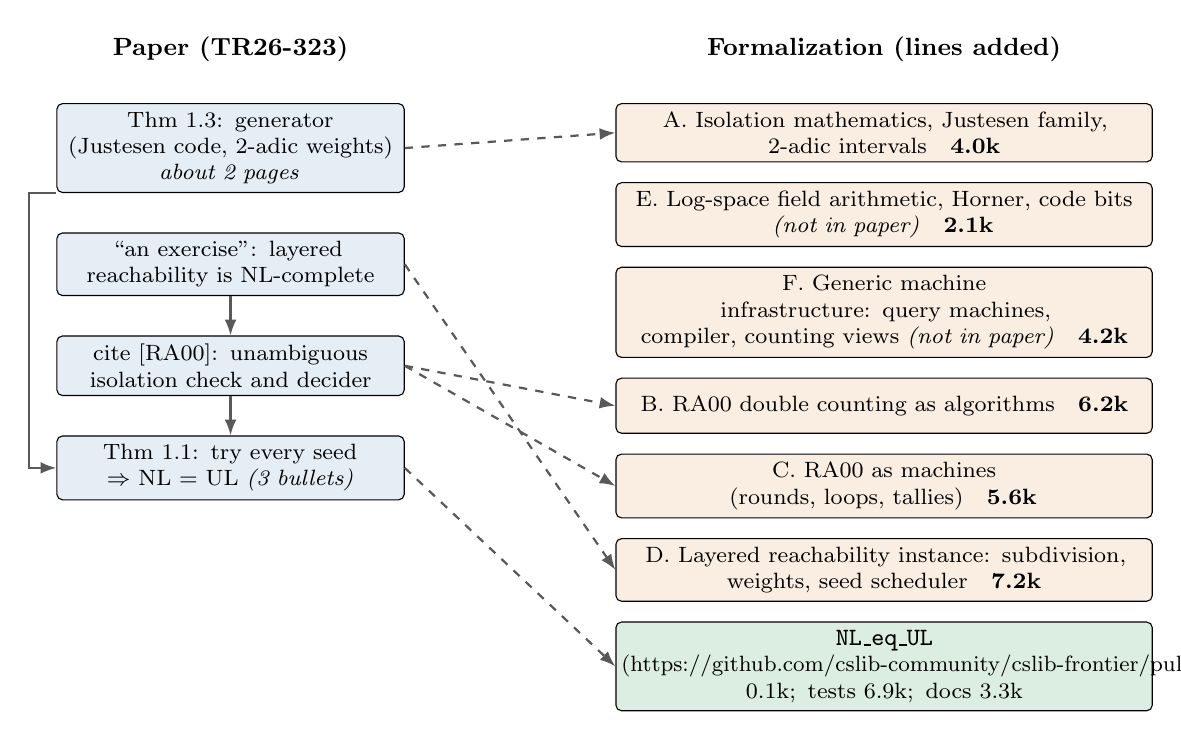
\begin{tikzpicture}[
  box/.style={draw,rounded corners=2pt,align=center,font=\footnotesize,execute at begin node={\hyphenpenalty=10000\exhyphenpenalty=10000},minimum height=7mm,inner sep=3pt},
  paper/.style={box,fill=c1!12},
  formal/.style={box,fill=c2!14},
  arr/.style={-{Latex[length=2mm]},thick,gray!70!black}]
\node[font=\small\bfseries] (P) at (0,0.2) {Paper (TR26-323)};
\node[paper,below=4mm of P,text width=4.2cm] (p13) {Thm 1.3: generator\\ (Justesen code, 2-adic weights)\\ \emph{about 2 pages}};
\node[paper,below=5mm of p13,text width=4.2cm] (pex) {``an exercise'': layered\\ reachability is NL-complete};
\node[paper,below=5mm of pex,text width=4.2cm] (pra) {cite [RA00]: unambiguous\\ isolation check and decider};
\node[paper,below=5mm of pra,text width=4.2cm] (p11) {Thm 1.1: try every seed\\ $\Rightarrow$ NL = UL \emph{(3 bullets)}};
\draw[arr] (pex) -- (pra); \draw[arr] (pra) -- (p11);
\draw[arr] (p13.south west) -- ++(-0.35,0) |- (p11.west);

\node[font=\small\bfseries] (F) at (8.3,0.2) {Formalization (lines added)};
\node[formal,below=4mm of F,text width=6.6cm] (fA) {A. Isolation mathematics, Justesen family,\\ 2-adic intervals\quad\textbf{4.0k}};
\node[formal,below=2.5mm of fA,text width=6.6cm] (fE) {E. Log-space field arithmetic, Horner, code bits\\ \emph{(not in paper)}\quad\textbf{2.1k}};
\node[formal,below=2.5mm of fE,text width=6.6cm] (fF) {F. Generic machine infrastructure: query machines,\\ compiler, counting views \emph{(not in paper)}\quad\textbf{4.2k}};
\node[formal,below=2.5mm of fF,text width=6.6cm] (fB) {B. RA00 double counting as algorithms\quad\textbf{6.2k}};
\node[formal,below=2.5mm of fB,text width=6.6cm] (fC) {C. RA00 as machines (rounds, loops, tallies)\quad\textbf{5.6k}};
\node[formal,below=2.5mm of fC,text width=6.6cm] (fD) {D. Layered reachability instance: subdivision,\\ weights, seed scheduler\quad\textbf{7.2k}};
\node[formal,below=2.5mm of fD,text width=6.6cm,fill=c3!18] (fT) {\code{NL\_eq\_UL} (\pr{7163}) 0.1k;\enspace tests 6.9k;\enspace docs 3.3k};
\draw[arr,dashed] (p13.east) -- (fA.west);
\draw[arr,dashed] (pex.east) -- (fD.west);
\draw[arr,dashed] (pra.east) -- (fB.west);
\draw[arr,dashed] (pra.east) -- (fC.west);
\draw[arr,dashed] (p11.east) -- (fT.west);
\end{tikzpicture}
\caption{Paper structure (left) against formal layers (right). Dashed arrows show which formal
layers realize each paper step. The ``exercise'' and the RA00 citation account for layers B--D
(19\,000 lines). Layers E and F implement machine-level details that the paper does not discuss. Boxes are
ordered to align with the paper's steps.}
\label{fig:deps}
\end{figure}

\begin{table}[!htbp]
\centering\small
\begin{tabularx}{\textwidth}{@{}lrrL@{}}
\toprule
Layer & Lines & Share & Content and reuse outlook\\
\midrule
A Paper mathematics & 3\,977 & 10\% & 2-adic interval lemma, derivative bounds, collisions, all-pairs isolation, Justesen family. Reusable for other isolation results.\\
B RA00 algorithms & 6\,242 & 16\% & Streaming scans, bounded walks, membership tallies, controller clocks. Reusable for other inductive-counting proofs.\\
C RA00 machines & 5\,576 & 14\% & Source rounds, round loops, tallies, predecessor loops. Partly reusable.\\
D Reachability instance & 7\,207 & 18\% & Subdivision adjacency, Justesen-weighted queries, seed scheduler. Mostly specific to this proof.\\
E Machine arithmetic & 2\,118 & 5\% & $\mathbb{F}_{2^k}$ multiplication without tables, trial division, modulus search, Horner evaluation, code bits. Reusable for coding theory and derandomization.\\
F Generic machines & 4\,177 & 11\% & Nondeterministic query machines, branch and call replay, counting views, offsets, \code{USPACE}. Broadly reusable.\\
Tests (clients) & 6\,873 & 17\% & At least one client per public layer.\\
Registry, docs, imports & 3\,345 & 8\% & Results inventory, references, import aggregates.\\
\midrule
Total & 39\,544 & & 795 public theorems, 439 private declarations, 83 definitions, 55 structures.\\
\bottomrule
\end{tabularx}
\caption{Added lines by layer between \code{c74b96b5} and \code{5a621fa1}. These are upper bounds
classified by path. Layers E and F (about 6\,300 lines) are general infrastructure; layer B (about
6\,200 lines) is reusable counting machinery.}
\label{tab:layers}
\end{table}

\paragraph{Why so long for five pages?} The paper is short because it rests on RA00 and on
informal conventions such as ``computable in $O(\log(wn))$ space''. A machine-level library has
to make each of these explicit, as Table~\ref{tab:layers} shows. A single sentence of the paper,
``the output $\rho(x,v)$ can be computed using $O(\log(wn))$ bits of space'', produced all of
layer~E. The paper's mathematics was not the bottleneck: its core lemmas landed in \pr{6757} at
hour~4.8, and the remaining generator mathematics followed by about hour~26.

\section{Timeline}
\label{sec:timeline}

\begin{figure}[!htbp]
\centering
\begin{tikzpicture}
\begin{axis}[width=\textwidth,height=6.2cm,xmin=0,xmax=48,ymin=0,ymax=235,clip=false,
  xlabel={hours since issue opened (20 Nov 14:57 UTC)},ylabel={PRs},
  xtick={0,6,...,48},legend style={at={(0.03,0.62)},anchor=west},legend style={font=\footnotesize,draw=none,fill=none},
  tick label style={font=\footnotesize},label style={font=\footnotesize}]
\fill[c4,opacity=0.08] (axis cs:14,0) rectangle (axis cs:18,235);
\fill[c4,opacity=0.08] (axis cs:34.7,0) rectangle (axis cs:47.0,235);
\addplot[c1,thick] table[x=h,y=opened]{cum.dat};
\addplot[c2,very thick] table[x=h,y=merged]{cum.dat};
\legend{opened (cumulative),merged (cumulative)}
\draw[black!70,dashed] (axis cs:4.8,0) -- (axis cs:4.8,215);
\node[font=\scriptsize,anchor=west,fill=white,inner sep=1pt] at (axis cs:5.1,212) {\pr{6757} core lemmas};
\draw[black!70,dashed] (axis cs:37.8,0) -- (axis cs:37.8,170);
\node[font=\scriptsize,anchor=east,fill=white,inner sep=1pt] at (axis cs:37.5,150) {\pr{7211} last layer};
\draw[black!70,dashed] (axis cs:47.0,0) -- (axis cs:47.0,170);
\node[font=\scriptsize,anchor=east,fill=white,inner sep=1pt] at (axis cs:46.7,120) {\pr{7163} Thm 1.1};
\node[font=\scriptsize,c4] at (axis cs:16,8) {lull};
\node[font=\scriptsize,c4] at (axis cs:41,8) {final tail};
\end{axis}
\end{tikzpicture}
\caption{Cumulative PRs opened and merged. Shaded: a lull with no merges (hours 14--18) and the
final tail (from \pr{7163} being ready at hour 34.7 to its merge at hour 47.0).}
\label{fig:cum}
\end{figure}

\begin{figure}[!htbp]
\centering
\begin{tikzpicture}
\begin{axis}[width=0.94\textwidth,height=5cm,xmin=0,xmax=48,ymin=0,
  ybar,bar width=3pt,xlabel={hours since issue opened},ylabel={issue comments / hour},
  xtick={0,6,...,48},axis y line*=left,tick label style={font=\footnotesize},label style={font=\footnotesize}]
\addplot[fill=c1!60,draw=none] table[x=h,y=comments]{hourly.dat};
\end{axis}
\begin{axis}[width=0.94\textwidth,height=5cm,xmin=0,xmax=48,ymin=0,
  axis y line*=right,axis x line=none,ylabel={Lean CI run-hours / hour},tick label style={font=\footnotesize},label style={font=\footnotesize}]
\addplot[c2,thick,mark=none] table[x=h,y=leanmin]{hourly.dat};
\end{axis}
\end{tikzpicture}
\caption{Coordination traffic (bars: comments on \iss{6747} per hour) and CI load (line: Lean
CI run-hours started per hour on these branches). CI load peaked at hour~5, during the first
fan-out. Comments peaked at hours 28--31 (21 Nov 19:00--23:00 UTC), when the stacked layers were
being integrated.}
\label{fig:hourly}
\end{figure}

\begin{table}[!htbp]
\centering\small
\begin{tabularx}{\textwidth}{@{}llL@{}}
\toprule
Hours & Phase & Landmarks\\
\midrule
0--5 & Plan and mathematics & Issue opened with a package plan. Six isolation PRs were consolidated into \pr{6757} (core lemmas, a first double-counting layer); \pr{6758} reduced NL to implicit layered reachability.\\
5--14 & Broad fan-out & Weighted subdivision \pr{6761}; UL$\subseteq$NL \pr{6782}; acceptance read off a machine's first halt \pr{6783}; binary encoding of the scan's guesses; bounds for the counting controller; seed search; code parameters; compiler from unambiguous procedures to UL machines \pr{6858}.\\
14--18 & Lull & No merges (21 Nov, about 05:00--09:00 UTC). Stacks for field arithmetic and input dispatch waited on reviews.\\
18--28 & Machine components & Horner evaluation \pr{6908}; a machine computing all weights; predecessor counting; bounded walks \pr{6951}; membership tallies \pr{6954}; one counting round per source \pr{6958}; the multi-round controller \pr{6962}.\\
28--38 & Rollup integration & Eleven rollups (\pr{7024}--\pr{7211}) carried most stacked layers. Seed scheduler, scheduler traces and native counting landed.\\
38--47.7 & Wait for final merge & The final PR's tail began at 34.7; see Table~\ref{tab:tail}. \pr{7163} merged at 47.0. Rollup \pr{7476} (Theorem 1.3 certificate and a Mod$_k$L corollary) merged at 47.7.\\
\bottomrule
\end{tabularx}
\caption{Phases of the formalization.}
\label{tab:phases}
\end{table}

Figures~\ref{fig:cum} and~\ref{fig:hourly} and Table~\ref{tab:phases} give the arc. Parallel
fan-out worked: 62 PRs merged by hour~14, with a median open-to-merge time of 1.3~hours (90th
percentile 4.2~h, maximum 16~h). The critical path was a chain of dependent layers: scan, walk,
tally, round, loop, scheduler, count, then the theorem. Each link needed its own review, restack
and queue pass, so adding workers could not shorten it.

\section{Routes taken, changed and abandoned}
\label{sec:routes}

The mathematical route never changed; it is the paper's. Every course change concerned
\emph{how} to realize the paper on machines, or how to organize people and PRs
(Table~\ref{tab:routes}). No PR was abandoned outright: all 63 closed PRs landed through
consolidation (6, into \pr{6757}) or through rollups and other carrying PRs (57).

\begin{table}[!htbp]
\centering\small
\begin{tabularx}{\textwidth}{@{}>{\raggedright\arraybackslash}p{3.0cm}L >{\raggedright\arraybackslash}p{2.1cm}@{}}
\toprule
Decision point & What happened & Outcome\\
\midrule
Proof route & Hoza's route exactly: generator, layered reachability, RA00 double counting, seed loop. The alternative via Applebaum's NL$\subseteq\oplus$L was not pursued; NL$\subseteq$Mod$_k$L was later derived as a corollary (\pr{7183}). & Used\\
Seed enumeration & A materialized list of candidate seeds was replaced by a bounded counter (\pr{6809}), so the scheduler stores $O(\log n)$ bits. & Changed early\\
Field arithmetic & Table lookups were replaced by table-free multiplication, trial division, modulus search and Horner evaluation (\pr{6768}, \pr{6787}, \pr{6794}, \pr{6822}, \pr{6908}). & Changed; reusable\\
Context certificates & Fixed-context certificates (\pr{6785}) were followed by runtime loaders (\pr{6790}); a field context that its claim called ``conditional'' was rebuilt on the native modulus search (\pr{6932}). & Stepping stones kept\\
Compiler correctness & The UL compiler mishandled a machine that halts before its first choice, counting two accepting runs instead of one; a review of \pr{6757} flagged the case and \pr{6781} fixed it. & Bug caught\\
Citation accuracy & Review of \pr{7183} removed a false priority claim (Applebaum had already proved NL$\subseteq\oplus$L) and marked the library's $\oplus$L as a run-counting convention, not the cited path-counting model. & Error caught\\
Work packaging & Large package claims were split into one-theorem claims; one lane stopped without code and was released. & Changed\\
Integration & Per-layer stacked PRs gave way, from hour 28, to rollups verified by the restack checker. & Changed late\\
Class definitions & UL and \#L were ported from an earlier unmerged branch instead of being redefined (\pr{6782}). & Reuse\\
Duplicates & Two workers claimed the final theorem; one withdrew within two minutes (hour 34.6). \pr{7107} duplicated \pr{7108} (a scheduler bound) and was left open. & Minor waste\\
Manuscript access & Reviewers reported the paper's PDF as unreachable and tried a private hand-off. The cause was a user-agent filter. & False dead end\\
\bottomrule
\end{tabularx}
\caption{Routes taken, changed and abandoned.}
\label{tab:routes}
\end{table}

\paragraph{Dead ends that cost time.} Both real dead ends were operational, not mathematical.
\begin{itemize}
\item \textbf{Disk.} The shared filesystem ran out twice, at hours 3.6 and 5.3. At hour~3.6 three
newly started workers produced no code, two of them because the disk was full. Each worker had its
own checkout and build outputs.
\item \textbf{Manuscript.} For about 11 hours the source check of the final theorem was wrongly
treated as needing a private copy of the PDF (Section~\ref{sec:tail}).
\end{itemize}
In addition, one PR diff (\pr{7021}) showed 31\,663 added lines because its base branch was wrong.
The diff was noise, but it consumed review attention.

\section{Process: what the pipeline cost}
\label{sec:process}

\begin{figure}[!htbp]
\centering
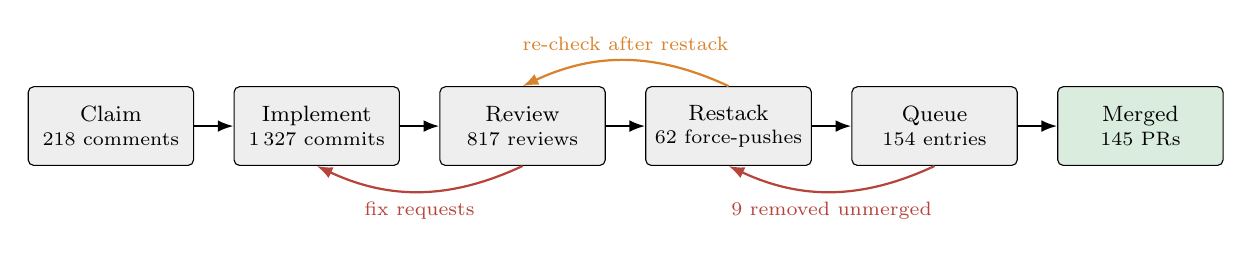
\begin{tikzpicture}[node distance=4mm and 5mm,
  st/.style={draw,rounded corners=2pt,fill=grayf,align=center,font=\footnotesize,minimum width=2.1cm,minimum height=10mm},
  arr/.style={-{Latex[length=2mm]},thick}]
\node[st] (a) {Claim\\[-1pt]\scriptsize 218 comments};
\node[st,right=of a] (b) {Implement\\[-1pt]\scriptsize 1\,327 commits};
\node[st,right=of b] (c) {Review\\[-1pt]\scriptsize 817 reviews};
\node[st,right=of c] (d) {Restack\\[-1pt]\scriptsize 62 force-pushes};
\node[st,right=of d] (e) {Queue\\[-1pt]\scriptsize 154 entries};
\node[st,right=of e,fill=c3!20] (f) {Merged\\[-1pt]\scriptsize 145 PRs};
\foreach \x/\y in {a/b,b/c,c/d,d/e,e/f} \draw[arr] (\x)--(\y);
\draw[arr,c4] (c.south) to[bend left=25] node[below,font=\scriptsize]{fix requests} (b.south);
\draw[arr,c4] (e.south) to[bend left=25] node[below,font=\scriptsize]{9 removed unmerged} (d.south);
\draw[arr,c2] (d.north) to[bend right=25] node[above,font=\scriptsize]{re-check after restack} (c.north);
\end{tikzpicture}
\caption{Life cycle of a component PR, with aggregate counts. Each landed lower layer forced the
layers above it to restack and be re-checked (orange loop). Rollups shortened this loop from
hour~28.}
\label{fig:pipeline}
\end{figure}

\begin{table}[!htbp]
\centering\small
\begin{tabularx}{\textwidth}{@{}lrL@{}}
\toprule
Measure & Value & Comment\\
\midrule
Wall clock & 47.0 / 47.7 h & To Theorem 1.1 / Theorem 1.3; component work ended at 37.8 h\\
PRs merged / closed / open & 145 / 63 / 1 & All closed PRs landed through consolidation, rollups or other carrying PRs\\
PRs per account & 132 / 62 / 15 & Three accounts, each running several agent workers\\
Submitted reviews & 817 & 5.6 per merged PR; 607 from the most active account's separate sessions\\
Issue comments & 615 & 396k characters, plus a 210k-character issue body\\
PR comments & 491 & \\
Force-pushes, base changes & 62, 13 & Restacks after lower layers landed\\
Merge-queue entries & 154 & 145 merged, 6 removed by hand, 2 conflicts, 1 invalid merge commit\\
Actions runs on these branches & 1\,712 & 11\,734 run-minutes (196 h)\\
Lean CI runs & 612 & 439 succeeded (7\,046 min), \textbf{163 cancelled (2\,057 min)}, 10 failed\\
Merge-group Lean runs & 150 & Median 17.2 min; 3\,398 min in total\\
Share of repository Lean CI & 22\% & 9\,172 of 41\,506 run-minutes in the window\\
\bottomrule
\end{tabularx}
\caption{Process and resource measures. Run-minutes are workflow wall time.}
\label{tab:process}
\end{table}

\subsection{Integration was the bottleneck}
Each layer was a separate PR stacked on the one below it (Figure~\ref{fig:pipeline},
Table~\ref{tab:process}). When a lower PR merged, every PR above it had to merge \code{main}, rerun
the restack checker, which carries the approval over if the diff is unchanged. It then
waited for CI before entering the queue. Each
queue pass cost a merge-group Lean run of about 17 minutes. With eight or more serial layers on
the critical path, queue and CI latency alone added several hours.

From hour~28, each rollup carried two to nine approved PRs. In hours 28--38, eleven rollup
merges landed 54 approved PRs that would otherwise each have needed its own queue pass. Figure~\ref{fig:cum}
counts a rollup as one merge, so it understates this. Had rollups been planned from hour~0,
most of the restack--re-check loop would never have run.

\subsection{Coordination traffic}
The issue served as both plan and ledger. Its body grew to 210\,000 characters, about 50\,000
tokens. Its 615 comments include 218 claims, 173 ``ready for review'' notes, 106 landing notes and
16 releases or withdrawals. Agents on recurring schedules reread this record to decide what to do;
according to local logs, some schedules fired every one or two minutes.

The claim protocol prevented almost all duplicated implementation. Its failures were small: the
duplicates in Table~\ref{tab:routes}, and one case where two sessions merged \code{main} into
\pr{7163} within seconds. One of them announced a head commit that was never pushed.

\subsection{CI and compute}
Of the 612 Lean CI runs, 163 (27\%) were cancelled because a newer push superseded them. They had
already used 2\,057 run-minutes, 22\% of Lean CI minutes on these branches. Merge-group runs used
3\,398 minutes. The Guide workflow, which by design runs whenever library sources change, added
2\,426 minutes. Locally, separate checkouts with separate build outputs repeated elaboration of
the same modules and filled the disk.

\subsection{The final 12 hours}\label{sec:tail}
Table~\ref{tab:tail} traces the tail of \pr{7163}. The proof was finished at hour~34.7; what
followed was gatekeeping and operations.

\begin{table}[!htbp]
\centering\small
\begin{tabularx}{\textwidth}{@{}llL@{}}
\toprule
UTC, 22 Nov & Hour & Event\\
\midrule
01:37 & 34.7 & \pr{7163} ready for review.\\
01:56 & 35.0 & Technical review approves; a check against the manuscript is still required.\\
02:06--02:30 & 35.2 & A reviewer asks whether the outside check read Theorem 1.1 in an identifiable copy. The publisher download is reported blocked, and a private hand-off fails.\\
03:37 & 36.7 & The author reports the patch re-verified on the updated \pr{7159} (no new head pushed).\\
04:44 & 37.8 & Last component layer \pr{7211} lands; \pr{7163} must restack again.\\
04:46--13:58 & 37.8--47.0 & No comments on the issue. Until about 09:00 the owning agent's provider was out of quota (local logs).\\
09:17 & 42.3 & \pr{7163} restacked after the owner was switched to another model; CI passes at 09:30.\\
09:30--12:57 & 42.5--46.0 & Waiting for the source check only.\\
12:57 & 46.0 & The coordinator reports that the server resets connections only from default \code{curl} and \code{python-requests} user agents; the public PDF matches the checksum.\\
13:04 & 46.1 & Outside-fleet source check of Theorem 1.1 passes.\\
13:06 & 46.2 & Two sessions merge \code{main} at once; a correction names the pushed head.\\
13:56 & 47.0 & \pr{7163} merges; \pr{7476} (Theorem 1.3) follows at 14:41.\\
\bottomrule
\end{tabularx}
\caption{The tail of the final theorem. About nine of its 12.3 hours were waiting. The quota
outage and the manuscript wait overlapped; the manuscript alone would have held the PR until
13:04.}
\label{tab:tail}
\end{table}

\subsection{Waste by dimension}
\label{sec:waste}
Table~\ref{tab:waste} separates the costs. Only wall-clock time and CI were measured directly.

\begin{table}[!htbp]
\centering\small
\begin{tabularx}{\textwidth}{@{}l>{\raggedright\arraybackslash}p{3.3cm}L@{}}
\toprule
Dimension & Measure & Main sources of waste\\
\midrule
Wall clock & 47.0 h; ${\sim}$9 h tail wait; 4 h lull & Serial queue passes, the manuscript misdiagnosis, the agent outage\\
CI & 11\,734 run-min; 2\,057 cancelled & Superseded pushes, per-layer merge-group runs, Guide runs on every library change\\
Agent tokens & Not metered & Rereading a 50k-token issue. Illustration: one schedule firing each minute for 48 h runs 2\,880 times; reading even a fifth of the issue each time is about 30M input tokens\\
Local CPU and disk & Not metered; disk full twice & Separate build outputs per checkout; repeated elaboration\\
Human attention & 615 comments, 817 reviews & Long narrative updates; re-running restack checks and re-announcing heads after each landing\\
\bottomrule
\end{tabularx}
\caption{Costs by dimension.}
\label{tab:waste}
\end{table}

\section{What could have been faster}
\label{sec:faster}

Table~\ref{tab:faster} lists changes that were available at the time. The savings are judgments
from the timeline, not measurements.

The 35-hour estimate is built as follows. Without the tail's waiting, \pr{7163} would have merged
about 1.5 hours after the last layer, at about hour~39. Rollups planned from the start would have
removed roughly three to five hours of serial restack, re-check and queue latency from the chain of dependent layers.
That gives about 34--36 hours for Theorem~1.1. The estimate keeps the 14--18 lull, since
contributors were less active then.

\begin{table}[!htbp]
\centering\small
\begin{tabularx}{\textwidth}{@{}L>{\raggedright\arraybackslash}p{2.6cm}>{\raggedright\arraybackslash}p{3.6cm}@{}}
\toprule
Change & Wall-clock saving & Other savings\\
\midrule
Record the manuscript checksum and a working download command when the issue opens & ${\sim}$4~h alone, ${\sim}$8~h with standby & Review rounds; hand-off attempts\\
Plan milestone rollups instead of per-layer queue passes & 3--5 h & ${\sim}$1\,500 merge-group minutes; most re-checks\\
Standby owner per endpoint and a second agent provider & ${\sim}$4 h (overlaps the first row) & No stalled restack\\
Batch fix-up pushes; avoid starting CI on heads that will be superseded & -- & Up to ${\sim}$2\,000 Lean CI minutes\\
Shared build cache and disk guards for worktrees & ${\sim}$1 h early & Local CPU; no disk exhaustion\\
Compact status table; slower schedules that wake on events & -- & Most reread tokens\\
Existing generic machine library (layers E, F) & days, for the next paper & ${\sim}$6\,300 lines now exist\\
\bottomrule
\end{tabularx}
\caption{Counterfactual savings. The rows overlap and do not add up.}
\label{tab:faster}
\end{table}

\section{Lessons learned}
\label{sec:lessons}

\begin{enumerate}
\item \textbf{Estimate from citations, not page count.} The paper's five pages hid RA00 and a
machine-level reduction. For a complexity paper, list the black boxes first and check which
already exist in the library.
\item \textbf{Fix the model contract early, then fan out.} The machine-class contract, the implicit
adjacency interface and the binary scan codec were agreed in the first hours. Later components
built on them without renegotiation. Shared interfaces found later, such as an offset-dispatch
API (\pr{6792}, hour~6) and a framed-header certificate (\pr{6928}, hour~20), were extracted
within minutes to hours.
\item \textbf{Parallelism helps the leaves, not the spine (the chain of dependent layers).} Breadth (arithmetic, codecs, bounds)
parallelized well. The dependent chain of scan, walk, tally, round, loop, scheduler and count did
not. Plan that chain explicitly and assign it reviewers who are online when each layer lands.
\item \textbf{Integrate in batches.} In hours 28--38, eleven rollup passes replaced 54
individual queue passes. Use rollups from the first stacked milestone.
\item \textbf{Keep the ledger small.} A 210k-character issue body is hard for people to read and
expensive for agents to reread. Keep a fixed-size status table (owner, branch, PR, state) and put
narrative in PRs.
\item \textbf{Avoid single points of failure.} One owner per endpoint without a standby, and one
agent provider without a fallback, stalled the final PR for about four hours. That stall
overlapped the manuscript wait.
\item \textbf{Treat source access as planning.} Record the paper's checksum and a reproducible
download command on day one. A ``connection reset'' from a tool is not evidence that a source is
unavailable.
\item \textbf{Make CI proportional.} Batch small fix-ups, avoid starting runs that will be
superseded, and scope expensive workflows to what a change can affect.
\item \textbf{Isolate workers, but share caches.} Separate checkouts are right for safety. Without
a shared build cache and disk guards, they multiply CPU and disk use.
\item \textbf{One head, one announcer.} After merging \code{main}, only the PR owner should push
and announce the new head; others should wait for the event.
\end{enumerate}

\paragraph{Follow-ups.} Concrete changes that would carry these lessons into the next issue:
\begin{itemize}
\item an issue template with fields for the paper checksum, a working download command, and an
owner plus a standby for each endpoint;
\item a fixed-size status table in the issue body, with narrative kept in PRs;
\item rollup tooling and a rule to roll up per milestone;
\item CI concurrency rules and path filters for expensive workflows;
\item a shared Lake build cache and a free-space guard for agent worktrees.
\end{itemize}

\section{Conclusions}

The formalization succeeded. Both theorems of TR26-323 hold for concrete log-space machines, with
exact counts of accepting runs and space bounds on every partial run, two days after the paper
appeared. The mathematical route held throughout. Both defects found, a compiler bug and a false
priority claim, were caught in review before merge.

Duration and cost came from two sources. The first is the gap between what a complexity paper may
cite and what a machine-level library must prove: roughly 90\% of the code. The second is a
process that parallelized component work well but serialized integration, coordination and the
final checks.

The first cost is partly paid for the future. About 6\,300 lines of general machine and arithmetic
infrastructure and about 6\,200 lines of reusable counting machinery are now on \code{main}. The
second cost can be cut with batch integration, a compact ledger, standby ownership, early source
verification and proportional CI.

\appendix
\section{Reproducing the measurements}

\code{collect.py} in this directory fetches the issue, the linked PRs (mentions in either
direction) and the Actions runs in the window, and writes \code{cum.dat} and \code{hourly.dat}.
Lines by layer come from \code{git diff --numstat c74b96b5 5a621fa1} over the 228 files touched
by merged PRs, classified by path:
\begin{itemize}
\item A: \code{MinIsolation}, \code{TwoAdic}, \code{JustesenFamily}, \code{Layered};
\item B: \code{DoubleCounting} outside \code{MultiTape};
\item C: \code{DoubleCounting} inside \code{MultiTape};
\item D: \code{STCON};
\item E: \code{InSpace}, \code{BinaryField}, \code{FieldTheory}, \code{Justesen};
\item F: other \code{MultiTape}, \code{Classes}, \code{Control}, \code{Data}, \code{Fin}.
\end{itemize}
These are dated observations at \code{5a621fa1}; do not update them in place.

\end{document}
